\documentclass[11pt,a4paper]{report}
\usepackage[utf8]{inputenc}
\usepackage[portuguese]{babel}
\usepackage[T1]{fontenc}
\usepackage[margin=2cm]{geometry}
\usepackage{graphicx}
\usepackage{amsmath}
\usepackage{csquotes}
\usepackage{enumitem}
\usepackage{listings}
\usepackage{listing}
\usepackage[svgnames]{xcolor}
\usepackage{eurosym}
\usepackage{csvsimple}
\usepackage{biblatex}
\usepackage{hyperref}
\usepackage{attachfile2}

\author{Carlos Pinto Machado
	<\href{mailto:2200909@estudante.uab.pt}{2200909@estudante.uab.pt}>}

\title{Exercícios Resolvidos da AULA AbERTA: Introdução à Estatística}

\addbibresource{./bibliografia.bib}
\makeindex
\lstset{
	language=R,
	basicstyle=\footnotesize,
	numbers=left,
	numberstyle=\tiny\color{gray},
	stepnumber=1,
	numbersep=5pt,
	backgroundcolor=\color{white},
	showspaces=false,
	showstringspaces=false,
	showtabs=false,
	frame=single,
	rulecolor=\color{black},
	tabsize=4,
	captionpos=b,
	breaklines=true,
	breakatwhitespace=false,
	keywordstyle=\color{blue},
	commentstyle=\color{DarkGreen},
	escapeinside={\%*}{*)},
	literate=
		{á}{{\'a}}1 {é}{{\'e}}1 {í}{{\'i}}1 {ó}{{\'o}}1 {ú}{{\'u}}1
		{Á}{{\'A}}1 {É}{{\'E}}1 {Í}{{\'I}}1 {Ó}{{\'O}}1 {Ú}{{\'U}}1
		{à}{{\`a}}1 {è}{{\`e}}1 {ì}{{\`i}}1 {ò}{{\`o}}1 {ù}{{\`u}}1
		{À}{{\`A}}1 {È}{{\`E}}1 {Ì}{{\`I}}1 {Ò}{{\`O}}1 {Ù}{{\`U}}1
		{ä}{{\"a}}1 {ë}{{\"e}}1 {ï}{{\"i}}1 {ö}{{\"o}}1 {ü}{{\"u}}1
		{Ä}{{\"A}}1 {Ë}{{\"E}}1 {Ï}{{\"I}}1 {Ö}{{\"O}}1 {Ü}{{\"U}}1
		{â}{{\^a}}1 {ê}{{\^e}}1 {î}{{\^i}}1 {ô}{{\^o}}1 {û}{{\^u}}1
		{Â}{{\^A}}1 {Ê}{{\^E}}1 {Î}{{\^I}}1 {Ô}{{\^O}}1 {Û}{{\^U}}1
		{ã}{{\~a}}1 {ẽ}{{\~e}}1 {ĩ}{{\~i}}1 {õ}{{\~o}}1 {ũ}{{\~u}}1
		{Ã}{{\~A}}1 {Ẽ}{{\~E}}1 {Ĩ}{{\~I}}1 {Õ}{{\~O}}1 {Ũ}{{\~U}}1
		{œ}{{\oe}}1 {Œ}{{\OE}}1 {æ}{{\ae}}1 {Æ}{{\AE}}1 {ß}{{\ss}}1
		{ű}{{\H{u}}}1 {Ű}{{\H{U}}}1 {ő}{{\H{o}}}1 {Ő}{{\H{O}}}1
		{ç}{{\c c}}1 {Ç}{{\c C}}1 {ø}{{\o}}1 {Ø}{{\O}}1 {å}{{\r a}}1 {Å}{{\r A}}1
		{€}{{\euro}}1 {£}{{\pounds}}1 {«}{{\guillemotleft}}1
		{»}{{\guillemotright}}1 {ñ}{{\~n}}1 {Ñ}{{\~N}}1 {¿}{{?`}}1 {¡}{{!`}}1
		{º}{\textdegree}1
}

\renewcommand*{\listlistingname}{Lista de Listagens}

\begin{document}
\maketitle
\tableofcontents

\clearpage

\chapter*{Introdução}\addcontentsline{toc}{chapter}{Introdução}

\paragraph{} No decorrer da AULA AbERTA - "Introdução à Estatística:
Estatística Descritiva com R"\cite{AulaAbertaIntroducaoEstatistica2017}, o
recurso formativo era um guia homónimo
\cite{OliveiraAulaAberta2017}, no qual existem
exercícios propostos. O presente documento pretende documentar soluções para o
mesmo com recurso à Bibliografia recomendada do mesmo
documento\cite{OliveiraEstatisticaDescritiva2011}.

\section*{Notas de Implementação}\addcontentsline{toc}{section}{Notas de Implementação}

\paragraph{} Para carregamento dos dados, foram utilizados ficheiros csv que
criam objectos dataframe. Esta abordagem parece ser mais razoável, dado que
podemos ter ficheiros com milhares de amostras.

\paragraph{} Em anexo, estão os recursos, código e datasets, em zip:
\attachfile[icon=Paperclip]{recursos.zip}

\clearpage

\setcounter{chapter}{2}
\chapter{Estatística Descritiva com R}
\section{Organização de dados no R}

\begin{table}[h!]
	\centering
	\begin{tabular}{|c|c|c|}
		\hline
		$x_i$&$n_i$&$f_i$ \\
		\hline
		0&11&0.275\\
		\hline
		1&16&0.400\\
		\hline
		2& 9&0.225\\
		\hline
		3& 2&0.050\\
		\hline
		4& 2&0.050\\
		\hline
	\end{tabular}
	\caption{Exercício 3.1 - Frequências simples e relativas de irmãos}
	\label{tab:3.1}
\end{table}
\lstinputlisting[caption={ex3\_1.R}]{./recursos/ex3_1.R}

\clearpage

\section{Visualização de dados usando o R}

\begin{figure}[h!]
	\centering
	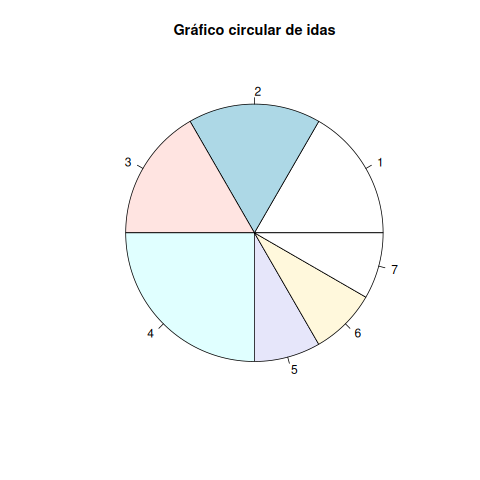
\includegraphics[width=0.4\textwidth]{./recursos/ex3_2.png}
	\caption{Exercício 3.2 - Gráfico circular de idas ao supermercado}
\end{figure}
\lstinputlisting[caption={ex3\_2.R}]{./recursos/ex3_2.R}

\clearpage
\section{Redução de dados: média aritmética e desvio padrão}

\begin{align*}
	\overline{x} &= 1.2\\
	s &\approx 1.067 \\
	\frac{s}{\overline{x}} &\approx 0.889 = 88.9 \%
\end{align*}

\paragraph{} A média permite-nos localizar a tendência central em redor dos
1.2 irmãos, e o desvio padrão de aproximadamente 1.067, permite-nos verificar
a dispersão associada. Sendo que o quociente do desvio padrão para com a média
é relativamente alto, permite-nos concluir que o esbatimento da curva é
rápido.

\paragraph{} Podemos verificar no gráfico \ref{fig:ex3_3} esse facto. Aparecem
também duas linhas a vermelho, demonstrando o conjunto de amostras no
intervalo com centro na média e raio de cumprimento do desvio
padrão($\overline{x} \pm s$). Data a natureza discreta da amostra fez-se uns
ajustes, sendo o intervalo dado por:
$[\lceil \overline{x} - s \rceil, \lfloor \overline{x} + s \rfloor]$.

\vspace{0.5cm}

\lstinputlisting[caption={ex3\_3.R}]{./recursos/ex3_3.R}


\begin{figure}[h!]
	\centering
	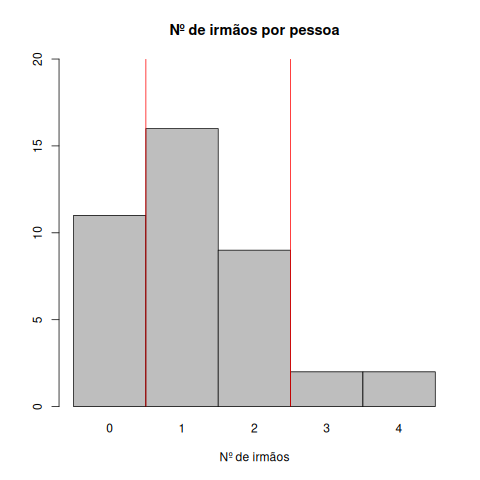
\includegraphics[width=0.4\textwidth]{./recursos/ex3_3.png}
	\caption{Exercício da secção 3.3 - Distribuição de irmãos por pessoa}
	\label{fig:ex3_3}
\end{figure}

\clearpage
\chapter{Exercícios}
\section*{Exercícios Propostos}

\begin{enumerate}[label=\arabic{chapter}.\arabic*]
	\item \addcontentsline{toc}{section}{4.1}
		\begin{enumerate}[label=\alph*)]
		\item $\overline{x} = 19.41667$\hfill
			\lstinputlisting[caption={ex4\_1a.R}]{./recursos/ex4_1a.R}
		\item $s = 1.378954$\hfill
			\lstinputlisting[caption={ex4\_1b.R}]{./recursos/ex4_1b.R}
		\end{enumerate}
	\item \addcontentsline{toc}{section}{4.2}\hfill
		\begin{enumerate}[label=\alph*)]
		\item $N = 60$\hfill
			\lstinputlisting[caption={ex4\_2a.R}]{./recursos/ex4_2a.R}
		\item \hfill
			\begin{table}[h!]
				\centering
				\begin{tabular}{|c|c|c|c|}
					\hline
					$x_i$&$n_i$&$N_i$&$f_i$ \\
					\hline
					1000&10&10&0.1666667\\
					\hline
					1100& 8&18&0.1333333\\
					\hline
					1200&12&30&0.2000000\\
					\hline
					1300& 8&38&0.1333333\\
					\hline
					1400&10&48&0.1666667\\
					\hline
					1500&12&60&0.2000000\\
					\hline
				\end{tabular}
				\caption{Tabela de 4.2 b)}
			\end{table}
			\lstinputlisting[caption={ex4\_2b.R}]{./recursos/ex4_2b.R}
			\clearpage
		\item \hfill
			\begin{align*}
				\overline{x} &= 1260 \\
				s &= 54.5552122756449
			\end{align*}
			\lstinputlisting[caption={ex4\_2c.R}]{./recursos/ex4_2c.R}
		\item \hfill
			\begin{figure}[h!]
				\centering
				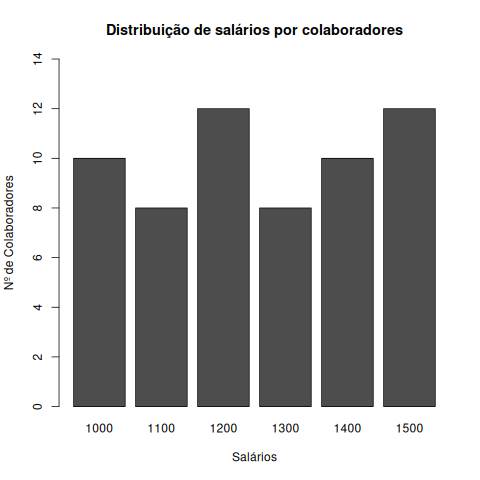
\includegraphics[width=0.4\textwidth]{./recursos/ex4_2d.png}
				\caption{Exercício 4.2 d) - Distribuição dos salários por nº de colaboradores}
			\end{figure}
			\lstinputlisting[caption={ex4\_2d.R}]{./recursos/ex4_2d.R}
		\end{enumerate}
		\item \addcontentsline{toc}{section}{4.3}\hfill
		\begin{enumerate}[label=\alph*)]
		\item $\overline{x} = 64.26667$\hfill
			\lstinputlisting[caption={ex4\_3a.R}]{./recursos/ex4_3a.R}
		\item $s = 9.676678$\hfill
			\lstinputlisting[caption={ex4\_3b.R}]{./recursos/ex4_3b.R}
		\end{enumerate}
		\clearpage
	\item \addcontentsline{toc}{section}{4.4}\hfill
		\begin{enumerate}[label=\alph*)]
		\item \hfill
			\begin{figure}[h!]
				\centering
				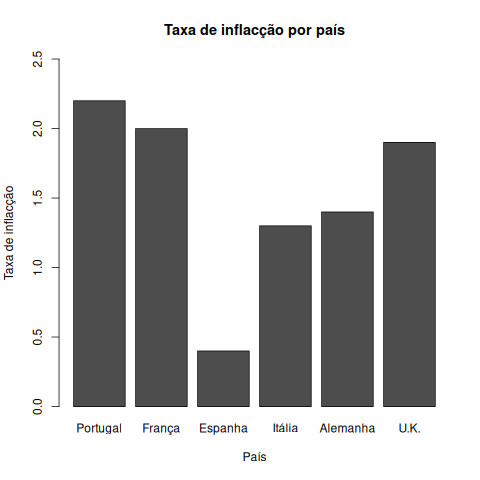
\includegraphics[width=0.4\textwidth]{./recursos/ex4_4a.png}
				\caption{Exercício 4.4 a) - Taxa de Inflação por país}
			\end{figure}
			\lstinputlisting[caption={ex4\_4a.R}]{./recursos/ex4_4a.R}
		\clearpage
		\item \hfill
			\begin{figure}[h!]
				\centering
				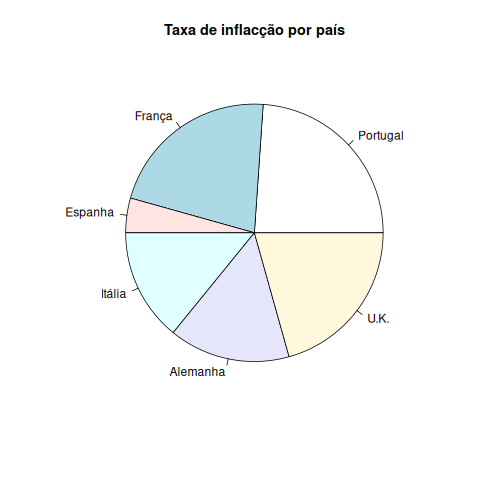
\includegraphics[width=0.4\textwidth]{./recursos/ex4_4b.png}
				\caption{Exercício 4.4 b) - Taxa de inflação por país(Gráfico
				circular)}
			\end{figure}
			\lstinputlisting[caption={ex4\_4b.R}]{./recursos/ex4_4b.R}
		\item $\overline{x} = 1.533333$\hfill
			\lstinputlisting[caption={ex4\_4c.R}]{./recursos/ex4_4c.R}
		\end{enumerate}
\end{enumerate}

\clearpage
\printbibliography[heading=bibintoc,title={Bibliografia}]
\listoftables\addcontentsline{toc}{chapter}{Lista de Tabelas}
\listoffigures\addcontentsline{toc}{chapter}{Lista de Figuras}
\listoflistings\addcontentsline{toc}{chapter}{Lista de Listagens}

\appendix

\chapter{Datasets}

\begin{table}[ht!]
	\begin{minipage}[t]{0.4\textwidth}
		\centering
		\csvautotabular{./recursos/dataset/4_1.csv}
		\caption{Autonomia(h) de smartphones\\ Ficheiro: 4\_1.csv}
	\end{minipage}\quad
	\begin{minipage}[t]{0.5\textwidth}
		\centering
		\csvautotabular{./recursos/dataset/4_2.csv}
		\caption{Salários (\euro) dos colaboradores\\ Ficheiro: 4\_2.csv}
	\end{minipage}
\end{table}
\begin{table}[ht!]
	\begin{minipage}[t]{0.4\textwidth}
		\centering
		\csvautotabular{./recursos/dataset/4_3.csv}
		\caption{Amostra - Peso(Kg) de alunos\\ Ficheiro: 4\_3.csv}
	\end{minipage}\quad
	\begin{minipage}[t]{0.4\textwidth}
		\centering
		\csvautotabular{./recursos/dataset/4_4.csv}
		\caption{Taxa de inflação por países \\ Ficheiro: 4\_4.csv}
	\end{minipage}
\end{table}
\begin{table}[t]
	\begin{minipage}[t]{0.4\textwidth}
		\centering
		\csvautotabular{./recursos/dataset/idas.csv}
		\caption{Idas ao supermercado\\ Ficheiro: idas.csv}
	\end{minipage}
	\begin{minipage}[t]{0.4\textwidth}
		\centering
		\csvautotabular{./recursos/dataset/irmaos.csv}
		\caption{Amostra - nº de irmãos\\ Ficheiro: irmaos.csv}
	\end{minipage}
\end{table}


\end{document}
